\documentclass[xcolor=pdftex,dvipsnames]{beamer}

\usepackage{amsmath}
\usepackage{amssymb}
\usepackage{comment}
\usepackage{textcomp}

\title{Microeconomic Theory --- ECON 323 503 \\ Chapter 6: Firms and Production}
\author{Vikram Manjunath}
\institute{Texas A\&M University}
\setbeamertemplate{navigation symbols}{}
\setbeamertemplate{footline}{}
\usefonttheme{serif}
\begin{document}

\maketitle

\begin{frame}
\frametitle{Outline}
\begin{enumerate}[<+->]
\item The ownership and management of firms: Who owns the firm and
  makes decisions about what/how much to produce?
\item Production: What are the firms possible choices?
\item Short-run production: Only some of the inputs can be varied. 
\item Long-run production: All of the inputs can be varied.
\item Returns to scale: Does output double when inputs are doubled?
\item Productivity and technical change: output changes with
  time for fixed amount of input.
\end{enumerate}
\end{frame}

\begin{frame}
\frametitle{Kinds of firms}
\begin{enumerate}[<+->]
\item Private sector: Owned by individuals and seek to maximize
  profits. Majority of GDP comes from such firms.
\item Public sector: Owned by the government. 
\item Non-profit: Not owned by government, but pursue social objectives.
\end{enumerate}
\end{frame}


\begin{frame}
\frametitle{Ownership of for-profit firms}
\begin{enumerate}
[<+->]
\item Sole proprietorship: Owned by an individual who is solely
  liable for the firm's debts.
\item Partnerships: Owned by two or more people who are liable for the
  firm's debts.
\item Corporations: Owned \emph{shareholders} who are not liable for
  the firm's debts.
\end{enumerate}

\end{frame}



\begin{frame}
\frametitle{Limited liability}
Shareholders in a corporation cannot be held responsible for its
debts.


\uncover<2->{Their personal assets are not used to pay those debts. They can only
lose what they paid for shares in the company (when the share price drops).}

\uncover<3->{\bigskip
This allows firms to raise funds and take risks that wouldn't be
possible under the other ownership structures.}

\end{frame}




\begin{frame}
\frametitle{Decision making}
Typically the ownership of a firm appoints the management.
\bigskip

\uncover<2->{Management's goal is (\emph{supposed to be}) to make decisions in the
owners' interest.}

\bigskip
\uncover<3->{We will ignore the fact that this isn't often the case in reality.}


\end{frame}




\begin{frame}
\frametitle{The owners' interest}
Profit maximization.
\bigskip

\uncover<2->{Profit ($\pi$) is the difference between revenue ($R$) and cost ($C$).
\[
\pi = R-C.
\]
$R$---what the firm earns from selling goods. 

If there's only one
good: $R=pq$.

\bigskip
$C$---what the inputs of producing the goods cost.}

\end{frame}




\begin{frame}
\frametitle{Efficient production}
To maximize profit, the firm must produce its output using the least
amount of input. 
\bigskip

\uncover<2->{Obvious that this is a \emph{necessary condition} for profit maximization.
\bigskip}

\uncover<3->{Not a \emph{ sufficient condition} though: the output level needs to
be right as well.}
\end{frame}




\begin{frame}
\frametitle{Production}
Categories of input:
\begin{enumerate}[<+->]
\item Capital (K): long-term inputs. E.g. Land, buildings,
  equipment.
\item Labor (L): hours of work provided by managers, skilled-workers,
  and unskilled-workers. 
\item Material (M): raw inputs. E.g. wood for a paper company.
\end{enumerate}
\end{frame}




\begin{frame}
\frametitle{Production functions}
Given certain amounts of inputs, what is the most output that a firm
can produce?
\bigskip

\uncover<2->{If a firm uses only capital and labor,
\[
q=f(L,K)
\]}

\end{frame}




\begin{frame}
\frametitle{Variability of inputs over time}
Short run:
\bigskip

\uncover<2->{Some inputs can't be changed (can't build a factory
overnight). These are \emph{fixed inputs} (or fixed factors).}
\bigskip

\uncover<3->{Others can be varied. These are \emph{variable inputs} (of variable
factors).}

\bigskip

\uncover<4->{Long run:
Everything is variable.}
\end{frame}




\begin{frame}
\frametitle{Short-run production}
We'll assume that there are two factors to production: K and L. 
\bigskip

\uncover<2->{K is fixed in the short run while L is variable.}
\bigskip

\uncover<3->{K is fixed at the level $\overline K$.}
\bigskip


\uncover<4->{Short run production function only depends on L:
\[
q=f(L,\overline K).
\]}
\uncover<5->{This is the \emph{total product of labor.}}

\end{frame}




\begin{frame}
\frametitle{Marginal product}
Total output from $L$ units of labor is $q=f(L, \overline K)$,
\bigskip

\uncover<2->{
What is the \emph{marginal} output from an additional unit of labor? }
\bigskip

\uncover<3->{The \emph{marginal product of labor}:
\[
MP_L = \frac{\delta q}{\delta L} = \frac{\delta f(L,\overline K)}{\delta L}.
\]}

\end{frame}




\begin{frame}
\frametitle{Average product}
What is the \emph{average} output from each unit of labor being used?

\bigskip
\uncover<2->{The \emph{average product of labor}:
\[
AP_L = \frac{q}{L} = \frac{f(L,\overline K)}{L}.
\]}
\end{frame}




\begin{frame}
\frametitle{The relationship between $MP_L$ and $AP_L$}
\begin{center}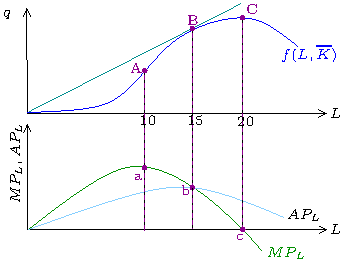
\includegraphics{pics/MPAP}\end{center}
Total output increases up to 20 units of labor and then decreases.
\end{frame}

\begin{frame}
\frametitle{The relationship between $MP_L$ and $AP_L$}
\begin{center}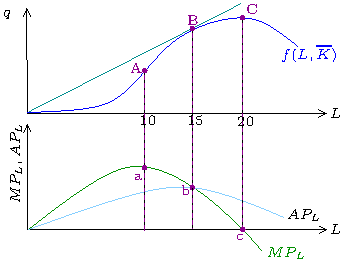
\includegraphics{pics/MPAP}\end{center}
Typically $AP_L$ rises (due to specialization) and then falls (because
other
factors are limiting). 
\end{frame}

\begin{frame}
\frametitle{The relationship between $MP_L$ and $AP_L$}
\begin{center}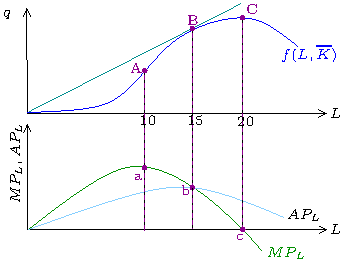
\includegraphics{pics/MPAP}\end{center}
Beyond 15 units of labor, the increase in total output is less than in
proportion to labor. So $AP_L$ falls.
\end{frame}


\begin{frame}
\frametitle{The relationship between $MP_L$ and $AP_L$}
\begin{center}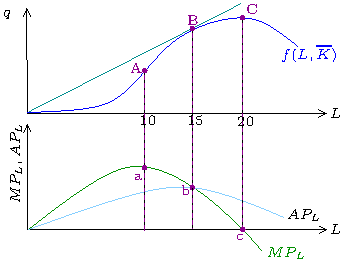
\includegraphics{pics/MPAP}\end{center}
If $MP_L > AP_L$, $AP_L$ is increasing: an additional unit of
labor is more productive than average. So the new average is higher.
\end{frame}


\begin{frame}
\frametitle{The relationship between $MP_L$ and $AP_L$}
\begin{center}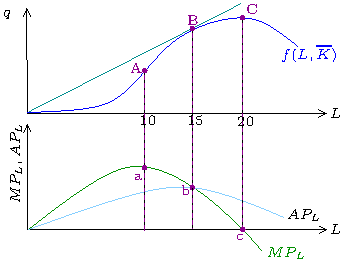
\includegraphics{pics/MPAP}\end{center}
If $MP_L < AP_L$, $AP_L$ is decreasing: an additional unit of
labor is less productive than average. So the new average is lower.
\end{frame}



\begin{frame}
\frametitle{The relationship between $MP_L$ and $AP_L$}
\begin{center}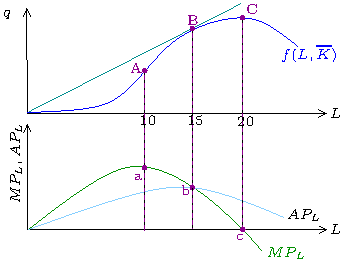
\includegraphics{pics/MPAP}\end{center}
$AP_L$ is the slope of the straight line from the origin to the total
product of labor. This is highest at point B.
\end{frame}


\begin{frame}
\frametitle{The relationship between $MP_L$ and $AP_L$}
\begin{center}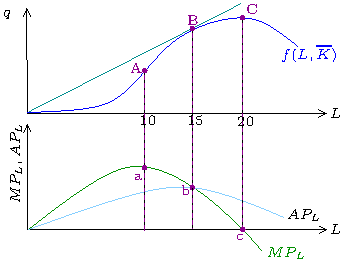
\includegraphics{pics/MPAP}\end{center}
$MP_L$ is the slope of the tangent to the total
product of labor. It is increasing until A and then starts to fall.
\end{frame}




\begin{frame}
\frametitle{Law of diminishing marginal returns}
This is a ``law'' in the same way as the ``law of demand'': it's an
empirical regularity.

\bigskip
\uncover<2->{\emph{If a firm keeps increasing an input without changing the others,
  or technology, the increases in output eventually become smaller.}
}

\bigskip
\uncover<3->{In other words: $MP_L$ eventually diminishes.}

\bigskip
\uncover<4->{Mathematically:
\[
\frac{\delta MP_L}{\delta L} = \frac{\delta\left(\frac{\delta q}{\delta
      L}\right)}{\delta L} = \frac{\delta^2 q}{\delta L^2} =
\frac{\delta^2 f(L,\overline K)}{\delta L^2} <0.
\]}

\end{frame}

\begin{frame}
\frametitle{Diminishing marginal returns}
This is not to be confused with ``diminishing returns.''
\bigskip

\uncover<2->{That would mean that as you increase $L$, total output decreases.}

\bigskip
\uncover<3->{There is no ``law of diminishing returns.''}
\end{frame}





\begin{frame}
\frametitle{Long-run production}
Both K and L can be varied. 
\bigskip

\uncover<2->{
There's more than one way to produce the same amount of output.}
\bigskip

\uncover<3->{More labor can make up for less capital and vice versa.}
\bigskip

\uncover<4->{Example: \[
q=L^{0.5}K^{0.5}
\]
For a fixed $\overline q$ we can draw a line through every pair of L
and K that yields $\overline q$ units of output.}

\bigskip
\uncover<5->{Each of (1,36), (2,18), (3,12),(4,9),(6,6),(9,4),(12,3),(18,2), and
(36,1) yield 6 units of output.}


\end{frame}




\begin{frame}
\frametitle{Isoquants}
\begin{center}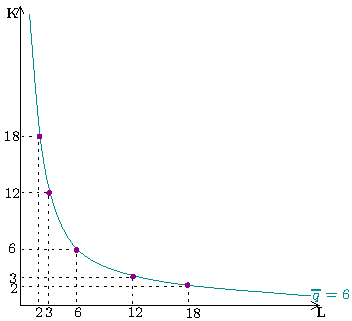
\includegraphics{pics/Isoquant1}\end{center}
The isoquant is a curve through all of those points.
\end{frame}


\begin{frame}
\frametitle{Isoquants}
\begin{center}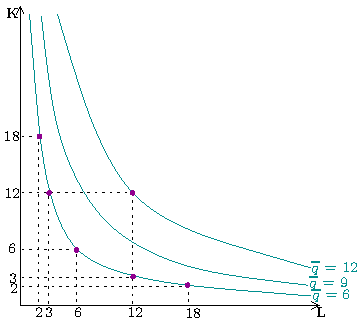
\includegraphics{pics/Isoquant2}\end{center}
For higher values of $\overline q$ we get higher isoquants.
\end{frame}



\begin{frame}
\frametitle{Properties of isoquants}
Much like indifference curves, they
\begin{enumerate}[<+->]
\item correspond to higher levels as you move $\nearrow$.
\item don't cross.
\item slope downwards.
\item are thin.
\end{enumerate}

\uncover<5->{
Biggest difference: the number associated with an isoquant (the
quantity produced) has  meaning, unlike utility which we can represent
using more than one function.
}
\end{frame}





\begin{frame}
\frametitle{Shapes of isoquants}
We saw the isoquants for Cobb-Douglas production.
\bigskip

\uncover<2->{
What about perfect substitutes? If you're making french fries,
potatoes from Idaho and potatoes from Maine are perfect substitutes.
\[
q = x+y.
\]}

\uncover<3->{Isoquant at $\overline q$ is given by pairs $(x,y)$ such that
$x+y=\overline q$. Or $y=\overline q - x$.}
\bigskip

\uncover<4->{Straight lines of slope -1 and intercept $\overline q$.}
\end{frame}






\begin{frame}
\frametitle{Isoquants: perfect substitutes}
\begin{center}
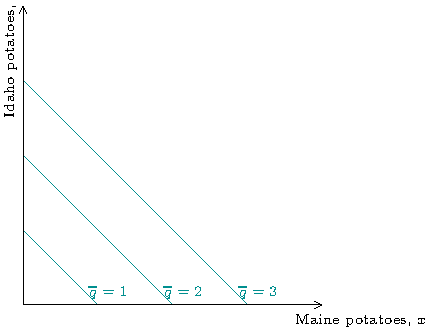
\includegraphics{pics/PerfSub}
\end{center}
\end{frame}


\begin{frame}
\frametitle{Shapes of isoquants}
What about perfect complements? \bigskip

\uncover<2->{If you're making computers you need processors and motherboards. 
\[
q=\min\{p,m\}.
\]}
\uncover<3->{
\begin{center}
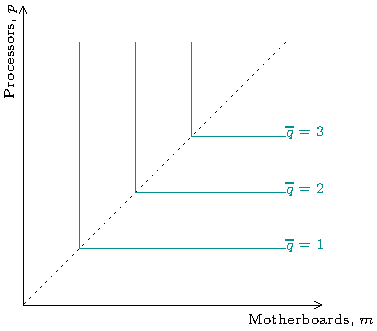
\includegraphics{pics/PerfComp}
\end{center}}


\end{frame}





\begin{frame}
\frametitle{Shapes of isoquants}
Of course, between these two extremes, we have \emph{imperfect}
substitution between inputs. As with Cobb-Douglas production.

\begin{center}
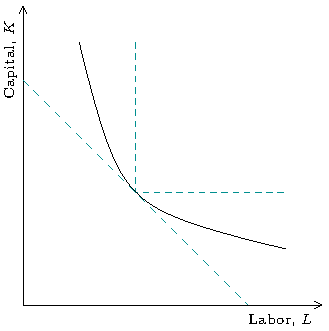
\includegraphics{pics/Imperf}
\end{center}


\end{frame}





\begin{frame}
\frametitle{Substituting Inputs}
The slope of an isoquant is the rate at which we can substitute one
input for another.

\bigskip
\uncover<2->{\emph{Marginal Rate of Technical Substitution}
\[
MRTS=\frac{\text{Change in capital}}{\text{Change in labor}} = \frac{dK}{dL}.
\]}
\uncover<3->{This is negative since isoquants slope downwards.}


\end{frame}

\begin{frame}
\frametitle{Substituting Inputs}
We can find MRTS by thinking about what happens to the amount of
$K$ needed if we increase $L$ by one unit but hold $\overline q$
fixed.
\bigskip

\uncover<2->{
$K(L)=$ Capital needed to produce $\overline q$ with $L$ units of labor.
}
\bigskip

\uncover<3->{Then \[\overline q = f(L, K(L)).\]}\uncover<4->{
Differentiating both sides of this equation with respect to $L$:
\[
\frac{d\overline q}{dL} = 0 = \frac{\delta f}{\delta L} + \frac{\delta
  f}{\delta K}\frac{dK}{dL} = MP_L + MP_K\frac{dK}{dL}.
\]}
\uncover<5->{
Rearranging this:
\[
MRTS = \frac{dK}{dL} = -\frac{MP_L}{MP_K}.
\]}
\end{frame}





\begin{frame}
\frametitle{Diminishing MRTS}
Just like MRS, MRTS tends to decrease as we move along an isoquant to
the right: The more you substitute one input for another, the more of
it you need.
\bigskip

\uncover<2->{When $f(L,K) = L^{0.5}K^{05}$, $MRTS=-\frac{K}{L}$.}


\bigskip

\uncover<3->{If we start substituting $L$ for $K$, $\frac{K}{L}$ grows, so the
isoquant gets flatter and flatter.}
\end{frame}






\begin{frame}
\frametitle{Returns to scale}
MRTS describes what happens when we keep output fixed and vary the
proportions of the inputs.
\bigskip

\uncover<2->{What happens as we increase all of the  inputs proportionally?\bigskip}

\bigskip
\uncover<3->{\emph{Constant returns to scale:} output increases proportionally with
input. For instance, $f(2L,2K) = 2f(L,K)$.}

\medskip
\uncover<4->{Replicable production processes would yield CRS. Just set up two
identical factories and you can double output.}

\bigskip
\uncover<5->{\emph{Increasing returns to scale:} output increases \emph{more than} proportionally with
input. For instance, $f(2L,2K) > 2f(L,K)$. }

\uncover<6->{Specialization can yield IRS: a bigger factory with more workers who
can specialize in their jobs can be more productive.}


\end{frame}






\begin{frame}
\frametitle{Returns to scale}

\emph{Decreasing returns to scale:} output increases \emph{less than} proportionally with
input. For instance, $f(2L,2K) < 2f(L,K)$.
\medskip

\uncover<2->{Models are abstractions. Unmodeled inputs are often limited and cause
decreasing returns to scale. For instance: you might run out of land
to build new factories on.}

\bigskip
\uncover<3->{\emph{Varying returns to scale}: The most usual situation is that production technology exhibits IRS
when output is low and DRS when it is high.}
\end{frame}






\begin{frame}
\frametitle{Productivity and technical change}
Technical progress and innovation cause increases in
productivity. What does this mean in our models?

\bigskip
\uncover<2->{
Suppose the production function is 
\[
q_1 = f(L,K).
\]}
\uncover<3->{

If a new invention causes a 10\% increase in productivity, the new
production function is
\[
q_2 = 1.1f(L,K).
\]}

\uncover<4->{This is a \emph{neutral} technical change since the firm can produce
more using the same ratio of inputs.}

\uncover<5->{A \emph{non-neutral} technical change would alter the ratios of the
inputs used.}
\end{frame}






\begin{frame}
\frametitle{Organizational changes}
Another way that a firm can become more productive is through
organizational changes. 

\bigskip
\uncover<2->{
Just yesterday HP decided to split into two
companies: one focusing on servers, software, and cloud tech and the
other on computers and printers.}
\bigskip

\uncover<3->{
HP shares are up 7.1\% today, reflecting that investors believe that
his will be a more productive organization of the firm.}


\end{frame}


\end{document}






